\section{Literature Review}

\subsection{Single Sign-On}
Single sign on (SSO) is an access technology that enables a user to sign on to any of their accounts through a single unified user interface \cite{sso1}. Without an SSO, users would have to sign on to each account using a specific username and password. SSO solutions should provide both security and convenience to an end user. Different types of SSO architectures exist, namely client side credential caching and server side credential caching. 

\subsubsection{Client-Side Credential Caching}
In client side credential caching all the authentication related information to various accounts is stored locally on the client side \cite{sso2}. This storage medium could be a database, or the local storage facility offered by modern browsers. A user operating under this SSO scheme expects to start the local SSO system once and then to have the relevant credential information automatically submitted during login. A software application (client) is also required to perform these duties as well as encrypt/decrypt credentials. 

The approach adopted in this report is to implement client-side credential caching based SSO through a browser extension. This is due to the fact that the end user of the system is not likely to have server level access to the end services. Additionally the use of a browser extension ensures that there is seamless integration with the user's browsing experience.

\subsubsection{Server-Side Credential Caching}
In contrast to client side credential caching, server side credential caching involves the storage of user credentials in a central repository on a remote server \cite{sso2}. The remote server is responsible for managing user authentication across multiple domains and services as apposed to a software client. This solution is ideal when a web administrator has access to multiple application servers that share a common authentication path.


\subsubsection{Kerberos Protocol }

Kerberos was one of the earliest single sign on solutions proposed within literature \cite{sso3}. The Internet Engineering Task Force (IETF) has defined Kerberos as an open standard and it is used widely for SSO authentication \cite{sso2}. Kerberos can be defined as a set of infrastructure that provides single sign on capabilities to network services. Kerberos infrastructure generally consists of an authentication server which is responsible for verifying a users claimed identity while the ticket generation server is responsible for providing authentication tokens to end users.  \clearpage

The authentication process for kerberos is initiated with a request from the client to the authentication server (middleman for a web service's particular credentials \cite{sso4}) for a pair of credentials. This set of credential information may be obtained from a centralized password database for example. The returned credentials will then consist of a server specific 'ticket' (generated by the ticket generation server) which uniquely identifies a particular user together with a temporary session (encryption) key. The client then transmits the ticket to the corresponding server of a web service. 

If the client is able to decrypt the ticket provided by the authentication server with the users unique password then it is assumed that the client has been authenticated. To further verify the users authenticity on the server side the end service decrypts the ticket provided by the client with a secret key, if this is possible then the client is assumed to be authentic.

\subsubsection{Conclusion}

Various SSO techniques exist, including both client side and server side credential storage and processing. Furthermore the kerberos protocol has been explored as the basis for SSO infrastructure and implementation. The approach adopted in this report will rely on a middle man client similar to the authentication server in kerberos. This client will interface with the browser extension and auxiliary micro-controller and be responsible for retrieving and decrypting credentials from storage as well as encrypting new credentials that are manually entered into a login portal.

\subsection{Password Managers}
Credentials fall into multiple categories. Usually authentication can either be based off something \cite{sso5}:
\begin{itemize}
  \item "you are" - such as biometrics
  \item "you know" - such as a PIN or password
  \item "you have" - such as an access card
\end{itemize}

For a long time, users have had to memorize a large array of username and password combinations. It then makes sense that as the number of credentials across multiple accounts increases, so too does the cognitive burden on the end user. Password managers rely on an electronic computing device, rather than a human to store credentials. Three broad categories of password managers exist, namely: desktop managers, portable managers and online managers \cite{sso5}. Online managers store passwords on third party servers while desktop managers store passwords on an end users computer. Finally portable password managers store passwords on a portable device such as a USB drive. The focus of this report is on developing a USB based portable password manager.

\subsubsection{User Behaviours}
For a long time, textual based passwords have been the defacto standard for online account security. It is generally recognized that humans fail to create strong, secure passwords \cite{sso6}. As a result various exploitation techniques targeted at compromising passwords such as brute forcing and man in the middle attacks are available to attackers.

In a study conducted by Karole et al. \cite{sso5} various participants were asked to rank the difficulty in using three types of password managers: phone based, USB based and online based. The results of the survey indicated that participants found the mobile phone based password the most difficult to use followed by the USB based password manager with the online password manager being ranked the easiest to use out of the three.

As a result the design of a portable (i.e USB based) password manager should provide a user friendly interface that makes password storage and maintenance easy for the end user. Besides the requirement to attach the device to the USB port of a computer, there should not be additional overhead in the process of storing passwords. 

\subsubsection{Features}

The core functionality of a password manager involves storing a users password and username in a central database\cite{sso7}. This database can exist locally or on a server. The database is also protected by a master key which should be kept secret so as to not compromise user credentials.

Modern password managers have a range of features these include: collaboration, encryption and login bookmarklets \cite{sso7}. Collaboration enables users to share passwords across computing devices while encryption functionality insures that credentials are stored in a format that is unintelligible and hard to decipher. Finally bookmarklets enable password managers to access the JavaScript context of a web page without requiring a browser extension during automatic field entry.

The approach adopted in this report however is to utilize a browser extension rather than a bookmarklet. This is due to the fact that bookmarklets are unable to provide a clear user interface component to the end user. Browser extensions allow for browser popups with which a suitable user interface to the end system can be presented to the end user.

\subsubsection{Threat Model}
Threat actors may be categorised by the level of resources available to them. Resources include computing capacity, as well as the availability of exploits or zero days. Threat actors may be individuals operating with limited resources or state actors with significant time and resources at their disposal. For the purposes of this report the main threat model will be assumed to be the web attacker. A web attacker could be described as an individual which has control over a number of web servers and can get a victim to connect to an attacker controlled server \cite{sso7}. It will also be assumed that a web attacker is able to develop a range of exploits that could be executed locally on a victims computing device (i.e code injection)
\subsubsection{Security}
Password managers have one key security objective, namely ensure that a stored credential is only accessed by an authorized individual and the corresponding website the credential belongs to. A variety of security goals for password managers exist\cite{sso7}, namely: master account security and credential database security.

With respect to the master account security, it is important that a password manager insure that an attacker can not simply emulate a user and decrypt credentials or obtain the master encryption key. For password managers that encrypt credentials it is important that the master key reside on the client side rather than a web interface to ensure that a web attacker can not obtain the master key as this would lead to credential exposure/leakage.

Credential database security should ensure that the medium through which credentials are stored is secured and that an attacker who has access to the credential database cannot simply extract sensitive information. For an encryption scheme such as RSA this means that private key information should not reside within the credential database. The credential database could be an SQL database or a filesystem on a microcontrollers EEPROM for example. Securely storing user credentials is one of the primary objectives of a password manager.

With regards to the attack surface of web based password managers four key vulnerabilities exist, namely: classic web vulnerabilities (such as cross site scripting, remote code execution, etc), authorization vulnerabilities, UI vulnerabilities and bookmarklet vulnerabilities. Portable password managers inherit a variety of security vulnerabilities especially when attacker is able to interfere at the client level, these include: password bruteforcing, code injection, malware and man in the middle attacks.

\subsubsection{Conclusion}
Various types of password managers exist. Password managers could be web based or hardware based (i.e USB based). Users often choose short insecure passwords when managing passwords themselves, password managers provide a solution to this problem. Password managers have a range of features which include encryption as well as credential autofill (bookmarklets). With regards to the threat model a realistic attacker is assumed to have both web based and local capabilities (which allow for techniques such as bruteforcing and code injection). 

Finally with regard to the security model, password managers should ensure both master account security and credential database security. 
\subsection{Password Compromise and Countermeasures}
Password security is a field within cybersecurity that focuses on the analysis and prevention of malicious disclosure of a user credential. This section of the literature review will focus on various methods/exploits targeted at compromising sensitive data such as credentials.

Various attack vectors exist which lead to credential leakage and mostly revolve around compromising data confidentiality and integrity \cite{embedded_security}.


\subsubsection{Code Injection}
Code injection relies on an information system executing attacker supplied, untrusted data within a process context. In the case of computing systems this attack is particularly effective at gaining control over a software client. These attacks may subsequently lead to password leakage.

An insertion vector or 'injector' is required when injecting attacker supplied code. In modern operating systems this may be through DLL (dynamic link library) injection \cite{game_hacking}, for JavaScript code injection this may be through the use of a browser extension or for an embedded system through the modification of a firmware EEPROM. 

Code injection allows for method detouring, a function hooking technique which allows an attacker to capture function call parameters at runtime. This may reveal sensitive information in the case of encryption functions such as the the encryption key used or plain-text data encrypted. Method detouring (shown in Figure 2.4) is achieved through patching specific assembly routines of a source function to call to a custom code section known as a detour function (shown in 1), which consists of a function prolog to save stack registers and call to an executable region known as a 'trampoline' (shown in 2). The trampoline contains the original opcode bytes that were patched in the source function along with a jump to the source function at a location just after the first jump to the detour function. The target function then returns control to the detour function (4) and finally the detour function, with a function epilog to restore the values of registers, jumps back the the original caller address (shown in 5)\cite{code_injection}.

Various techniques exist for preventing code injection including signature based methods to calculate an overall hash value for an executable module and compare its run time equivalent signature. Recent research by Wei Hu Et al. \cite{code_injection2} have proposed a mechanism known as software dynamic translation which is a form of instruction-set randomization and encryption to thwart generalized code injection attacks.

\begin{figure}[H]
\centering
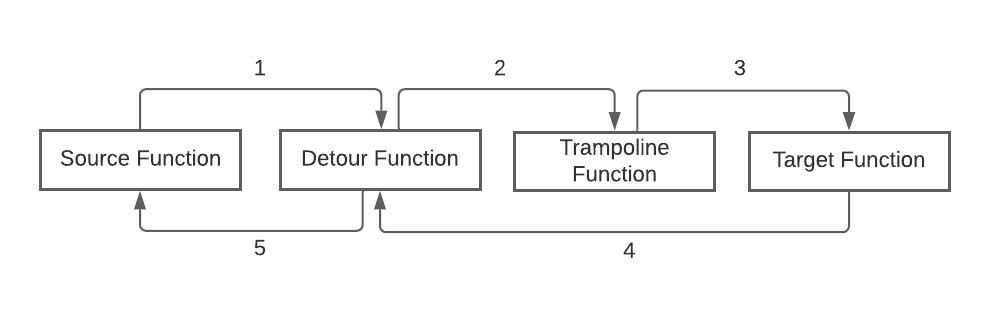
\includegraphics[width=0.8\columnwidth]{Figures/Fig_63.png}
\caption{Model for function detouring.  }
\label{fig:gantt}
\end{figure}

\subsubsection{Malware}

Malware is any software that is intentionally designed to have a malicious impact on an information system. The deployment of malware on a computing device by a threat actor may lead to the partial of complete compromise of the end system including sensitive data such as passwords. The distribution of malware may be through the use of social engineering or software or hardware compromise. The mode of operation of malware is typically through memory exploitation or code injection. Various malware variants exist, including \cite{malware}:

\begin{itemize}
  \item Viruses: The most generic form of malware. These are computer programs or software that is typically hidden within a legitimate piece of software to carry out a malicious or destructive function. 
  \item Trojan Horses: These are harmful software applications that misrepresent their identity to disguise themself as regular, benign programs. They usually carry a hidden destructive function which is activated when the software is executed for the first time.
   \item Rootkits: Rootkits are a specialized malware strain that often combine privilege escalation exploitation in order to make modification to system software such as an operating system or system firmware. They typically operate at the highest level of the access control chain of an information system. Modifications to system software are typically aimed at concealing malicious activity.
  \item Backdoors: An attacker may wish to gain remote access to an information system. In this case a strain of malware known as backdoors may be deployed to a target, often through the use of a compromised network channel. Backdoors are often stealthy in their operation and may typically lay dormant on a system for an extended period of time before the malware is activated through the use of a command and control server relay.
  \item Ransomware: A destructive form of malware that typically encrypts a file system and then prompts a victim for a payment to receive a decryption key and recover files. Ransomware may use sophisticated anti-evasion techniques to avoid detection.
  \end{itemize}
  
  
  Various countermeasures against malware exist including anti-virus software, which often uses signature based methods to identify malware strains. Additionally the use of a neural network heuristic engine that is self learning, is also common \cite{malware_2}. A heuristic engine uses machine learning and is responsible for identifying potential malicious activity in real time in the case where a particular malware variant has not had its signature captured, i.e has not been added to a master threat database.
 

\subsubsection{Conclusion}

Various end attack vectors exist which are aimed at disclosing sensitive information such as credentials. For software based exploitation this may include brute forcing credentials, exploiting system memory or injecting user supplied code. Additionally the placement of malware onto a computing system might grant an attacker remote access to a networked system or an attacker might monitor an information channel to exfiltrate or modify data destined for a receiver.  


\subsection{Password Encryption Standards}

Various methods have been proposed for ensuring credential security. The U.S. National Institute of Standards and Technology has historically played a key role in the development of modern, secure algorithmic standards for the encryption of data. Various symmetric and asymmetric encryption algorithms have been designed throughout the century\cite{encryption_standards} ranging from simple block ciphers, advanced elliptic curve based algorithms and even future, quantum resistant encryption standards.

This section of the literature review aims to explore modern encryption standards as applied to the protection of sensitive data such as credentials. Various performance metrics as applied to the analysis of encryption exist, including: encryption time, decryption time, memory consumption and data entropy.

\subsubsection{AES}

The advanced encryption standard (AES) is a symmetric block cipher developed by two Belgian cryptographers Joan Daemen and Vincent Rijmen. AES has a block size of 128 bits and three varying key sizes of 128, 192 and 256 bits respectively. It was chosen as a successor to the now insecure data encryption standard (DES). AES was subject to a committee based selection process from a range of competing algorithms including: MARS, RC6, Rijndael, Serpent and Twofish. Ultimately the Rijndael cipher was chosen and AES is also known by its original name, Rijndael \cite{encryption_standards}.

As apposed to a Feistel network, AES relies on a design principle known as a substitution-permutation network and its implementation is efficient in both hardware and software. Operations on bytes are through the use of a 4x4 matrix known as the state. The number of rounds of processing is dependant on the key size used with 10 rounds being required for 128-bit keys, 12 rounds for 192-bit keys and 14 rounds for 256-bit keys \cite{aes}.

\begin{figure}[H]
\centering
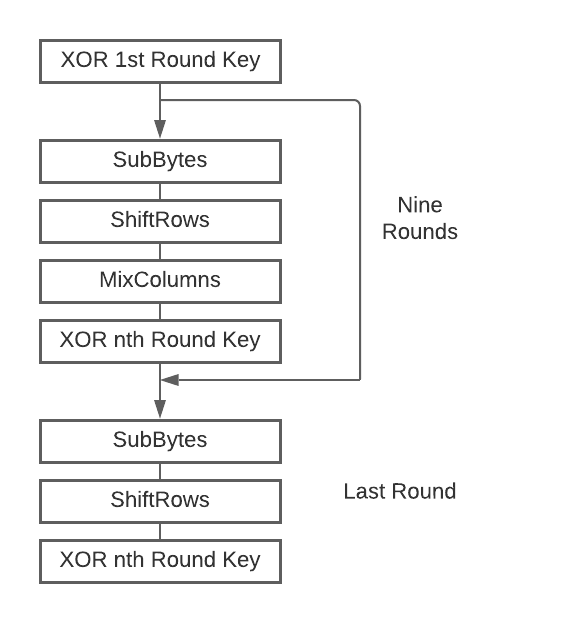
\includegraphics[width=0.5\columnwidth]{Figures/Fig_64.png}
\caption{AES-128 bit encryption high level overview.}
\label{fig:gantt}
\end{figure}

Figure 2.2 depicts a high level overview of the encryption steps for a keysize of 128-bits. Each round of processing consists of various steps \cite{aes}:
\begin{itemize}
  \item Expansion: Here the AES schedule is used to derive the various subkeys from the master key.
  \item AddRoundKey: The subkey and state matrix are added using an exlusive-or (XOR) operator.
  \item SubBytes: Bytes in the state matrix are then substituted using a non-linear transformation via a lookup table. 
   \item ShiftRows: The last three rows of the state matrix are shifted cyclically through a transposition step.
   \item MixColumns: Columns of the state matrix are mixed together where the four bytes in each column are combined.
  \end{itemize}

Research conducted by Abdulrahman Ali et al. \cite{aes_second} indicates that AES uses less memory than RSA during encryption and decryption. AES was also shown to be the fastest to decrypt a 3MB file when compared against RSA. However for small file sizes (around 25kB) there was no substantial change in decryption times. The additional complexity introduced through an AES implementation should thus be considered against simpler algorithmic implementations when selecting an encryption algorithm for password protection. 

AES is typically used in wireless security applications, processor security, SSL/TLS as well as file encryption.

\subsubsection{RSA}
RSA, named after its creators Ron Rivest, Adi Shamir and Leonard Adleman, is an asymmetric encryption algorithm developed in 1977. The algorithm makes use of four individual steps, namely: the generation of keys, the distribution of keys as well as encryption and decryption. The algorithm is based on the fact that finding the prime factors of a large composite number is particularly difficult.

As an asymmetric algorithm RSA involves the use of of a public and private key. The public key key may be distributed openly and used to encrypt information while the private key should be kept secret and is used to decrypt data. The public and private key are generated using the following algorithm \cite{encryption_standards}:

\begin{enumerate}
  \item Two large random prime numbers p and q are chosen.
  \item The modulus of the public and private keys (n) are calculated, $ n = pq $.
  \item Compute Eulers totient, $ \phi(n) = (p-1)(q-1) $ 
   \item An integer $ e $ is chosen such that $ 1 < e < \phi(n) $ and $e$ is coprime to $\phi(n)$
   \item Calculate $d $ satisfying the congruent relation $de = 1\,mod\, \phi(n)$.
  \end{enumerate}

$e$ is then the resulting public key exponent and d the private key exponent. A popular choice for the public key exponent is $e = 2^{16} + 1 = 65537$ although smaller values of e may also be used to speed up encryption signature verification \cite{rsakey} on certain resource limited embedded systems.

Assume a message transfer between two parties, Bob and Alice. Furthermore assume Bob gives his public key, presented by $n and e$ to Alice but keeps his private key a secret. Alice wishes to send a message, $m$, to Bob. The corresponding ciphertext $c$ can then be computed as follows:
\[ c = m^e\,mod\,n\]
Alice then sends $c$ to Bob. Bob is able to recover the original message (m) from c using his private key, d in the following relation:
\[ m = c^d\,mod\,n\]

RSA is still used in a wide range of applications ranging from web browsers, email and chat clients. RSA is also used to secure communications between VPN clients and servers. However as an asymmetric algorithm it is generally more computationally expensive both in terms of encryption/decryption times as well as memory consumption. However the implementation of RSA is rather straightforward compared to more advanced algorithms such as AES.  
